% \documentclass{article}
% \input{../preamble}
% \usetikzlibrary{math}
% \usepackage{cancel}

% \numberwithin{equation}{section}
% \setcounter{section}{6}
% \numberwithin{figure}{section}

% \usepackage{fancyhdr}
% \pagestyle{fancy}
% \renewcommand{\headrulewidth}{0pt}
% \renewcommand{\headruleskip}{0mm}
% \fancyfoot[C]{Access for free at \href{https://openstax.org/books/physics/pages/1-introduction}{https://openstax.org/books/physics/pages/1-introduction}
% \hfill \thepage}
% \fancyhead{}

% \title{Unit 6: 2D Motion}
% \author{Edited by Luis Nunez}
% \date{Updated on \today}

\documentclass[main.tex]{subfiles}

\begin{document}

\section{Force Interactions}

\subsection{Vectors and Components}

A vector is a quantity with a magnitude and direction. A vector is represented by an arrow of a certain size, pointing in a certain direction. Magnitude means the size (or length) of a vector. Direction is the angle ($\theta$) from the $x$-axis to a vector on the coordinate plane. See ``standard position'' below. Vectors represent physical quantities, like position, displacement, velocity, and acceleration. They are plotted on the $x$-$y$ coordinate plane. An arrow above a symbol, as in $\vec{A}$, represents the magnitude and direction for vector $A$; the letter by itself signifies magnitude only, not direction. For example,

\begin{equation*}
    \vec{A} = \SI{-6}{m}\ , \hspace{1em} A = \SI{6}{m}
\end{equation*}


The $x$-component (as in  $\vec{A}_x$) is the horizontal component of a vector; the projection of a vector on $x$-axis.


The $y$-component ($\vec{A}_y$) is the vertical component of a vector; the projection of a vector on $y$-axis.

\begin{example}
Consider vector $\vec{A}$ below. (a) What is $x$-component of vector $\vec{A}$? (b) What is the $y$-component?
\end{example}

\begin{figure}[h!]
    \centering
\def\Ax{6}
\def\Ay{4}
\begin{tikzpicture}
\pgfplotsset{compat=1.11}
    \begin{axis}[width=7cm,height=7cm,
        axis lines = middle,
        xlabel = $x$, x label style={anchor=west},
        ylabel = $y$, y label style={anchor=south},
        ymin=-8, ymax=8,
        xmin=-8, xmax=8,
        xtick={-8,-6,...,8},
        ytick={-8,-6,...,8},
        ymajorgrids=true,
        xmajorgrids=true,
        clip=false,
        ]
        \draw[ultra thick,red,->] (axis cs: 0,0) -- (\Ax,\Ay) node[red,above] {$\vec{A}$};
    \end{axis}
\end{tikzpicture}%
\hspace{2em}
\begin{tikzpicture}
\pgfplotsset{compat=1.11}
    \begin{axis}[width=8cm,height=8cm,
        axis lines = middle,
        axis line style={black!20},
        xlabel = $x$, x label style={anchor=west},
        ylabel = $y$, y label style={anchor=south},
        ymin=-8, ymax=8,
        xmin=-8, xmax=8,
        xtick={-8,-6,...,8}, xticklabels={,,},
        ytick={-8,-6,...,8}, yticklabels={,,},
        extra x ticks={6}, extra x tick labels={6},
        extra y ticks={4}, extra y tick labels={4},
        clip=false,
        ]
        \draw[thick,->] (0,0) -- (\Ax,0);
        \draw[thick,->] (\Ax,0) -- (\Ax,\Ay);
        \node[above] at (axis cs: \Ax*1.2/2,0) {$A_x$};
        \node at (axis cs: \Ax*1.1,\Ay/2) {$A_y$};
        \draw[ultra thick,red,->] (0,0) -- (\Ax,\Ay) node[red,above] {$\vec{A}$};
        \node at (-4,8) {\Solution}; 
    \end{axis}
\end{tikzpicture}
\end{figure}

The $x$-component is 6. The $y$-component is 4. See the graph above.

\clearpage

\begin{example}
Find the $x$-component ($\vec{A}_x$) and $y$-component ($\vec{A}_y$) of vector $\vec{A}$.
\end{example}

\begin{figure}[h!]
    \centering
\def\Ax{-7}
\def\Ay{3}
\begin{tikzpicture}
\pgfplotsset{compat=1.11}
    \begin{axis}[width=8cm,height=8cm,
        axis lines = middle,
        xlabel = $x$, x label style={anchor=west},
        ylabel = $y$, y label style={anchor=south},
        ymin=-8, ymax=8,
        xmin=-8, xmax=8,
        xtick={-8,-6,...,8}, 
        ytick={-8,-6,...,8}, 
        ymajorgrids=true,
        xmajorgrids=true,
        yminorgrids=true, minor y tick num=1,
        xminorgrids=true, minor x tick num=1,
        clip=false,
        ]
        \draw[ultra thick,red,->] (0,0) -- (\Ax,\Ay) node[above,red] {$\vec{A}$};
    \end{axis}
\end{tikzpicture}%
\hspace{2em}
\begin{tikzpicture}
\pgfplotsset{compat=1.11}
    \begin{axis}[width=8cm,height=8cm,
        axis line style={black!20},
        axis lines = middle,
        xlabel = $x$, x label style={anchor=west},
        ylabel = $y$, y label style={anchor=south},
        ymin=-8, ymax=8,
        xmin=-8, xmax=8,
        xtick={-8,-6,...,8}, xticklabels={,,},
        ytick={-8,-6,...,8}, yticklabels={,,},
        extra x ticks={\Ax}, extra x tick labels={\Ax},
        extra y ticks={\Ay}, extra y tick labels={\Ay},
        clip=false,
        ]
        \draw[ultra thick,red,->] (axis cs: 0,0) -- (\Ax,\Ay) node[above,red] {$\vec{A}$};
        \draw[thick,->] (0,0) -- (\Ax,0);
        \draw[thick,->] (\Ax,0) -- (\Ax,\Ay);
        \node[above] at (\Ax*1.2/2,0) {$A_x$};
        \node at (\Ax*1.1,\Ay/2) {$A_y$};
        \node at (-4,8) {\Solution};
    \end{axis}
\end{tikzpicture}
\end{figure}

The components are

\begin{equation*}
    \vec{A}_x = -7\ , \hspace{1em}
    \vec{A}_y = +3
\end{equation*}


\subsection{Angles and Standard Position}

Angles are graphed in one of the four quadrants in the coordinate plane. An angle in \href{https://openstax.org/books/algebra-and-trigonometry-2e/pages/7-1-angles}{standard position} has its vertex at the origin and its initial side on the $+x$ axis (or east direction). Positive angles are measured counter-clockwise from the $+x$ direction.

\begin{figure}[h!]
    \centering
    \def\A{2.5}
    \def\Q{2}
\begin{tikzpicture}
    \pgfplotsset{compat=1.11}
    \begin{axis}[width=5cm,height=5cm,
        axis lines=middle,
        axis line style={black!80},
        xmin=-3,xmax=3,ymin=-3,ymax=3,
        ticks = none,
        clip=false,
    ]
    \draw[very thick,->,blue] (0,0) -- (\A,0) node[above] {\SI{0}{\degree}};
    \node at (\Q,\Q) {\footnotesize \textbf{I}}; \node at (-\Q,\Q) {\footnotesize \textbf{II}}; \node at (-\Q,-\Q) {\footnotesize \textbf{III}}; \node at (\Q,-\Q) {\footnotesize \textbf{IV}};
    \end{axis}
\end{tikzpicture}%
\hspace{1em}
\begin{tikzpicture}
    \def\A{2.5}
    \pgfplotsset{compat=1.11}
    \begin{axis}[width=5cm,height=5cm,
        axis lines=middle,
        axis line style={black!80},
        xmin=-3,xmax=3,ymin=-3,ymax=3,
        ticks = none,
        clip=false,
    ]
    \draw[very thick,->,blue] (0,0) -- (\A,0);
    \draw[very thick,->,blue] (0,0) -- (0,\A) node[below left,blue] {\SI{90}{\degree}};
    \draw[->] (1,0) arc (0:90:1);
    \node at (\Q,\Q) {\footnotesize \textbf{I}}; \node at (-\Q,\Q) {\footnotesize \textbf{II}}; \node at (-\Q,-\Q) {\footnotesize \textbf{III}}; \node at (\Q,-\Q) {\footnotesize \textbf{IV}};
    \end{axis}
\end{tikzpicture}%
\hspace{1em}
\begin{tikzpicture}
    \def\A{2.5}
    \pgfplotsset{compat=1.11}
    \begin{axis}[width=5cm,height=5cm,
        axis lines=middle,
        axis line style={black!80},
        xmin=-3,xmax=3,ymin=-3,ymax=3,
        ticks = none,
        clip=false,
    ]
    \draw[very thick,->,blue] (0,0) -- (\A,0);
    \draw[very thick,->,blue] (0,0) -- (-\A,0) node[above,blue] {\SI{180}{\degree}};
    \draw[->] (1,0) arc (0:180:1);
    \node at (\Q,\Q) {\footnotesize \textbf{I}}; \node at (-\Q,\Q) {\footnotesize \textbf{II}}; \node at (-\Q,-\Q) {\footnotesize \textbf{III}}; \node at (\Q,-\Q) {\footnotesize \textbf{IV}};
    \end{axis}
\end{tikzpicture}%
\hspace{1em}
\begin{tikzpicture}
    \def\A{2.5}
    \pgfplotsset{compat=1.11}
    \begin{axis}[width=5cm,height=5cm,
        axis lines=middle,
        axis line style={black!80},
        xmin=-3,xmax=3,ymin=-3,ymax=3,
        ticks = none,
        clip=false,
    ]
    \draw[very thick,->,blue] (0,0) -- (\A,0);
    \draw[very thick,->,blue] (0,0) -- (0,-\A) node[above left,blue] {\SI{270}{\degree}};
    \draw[->] (1,0) arc (0:270:1);
    \node at (\Q,\Q) {\footnotesize \textbf{I}}; \node at (-\Q,\Q) {\footnotesize \textbf{II}}; \node at (-\Q,-\Q) {\footnotesize \textbf{III}}; \node at (\Q,-\Q) {\footnotesize \textbf{IV}};
    \end{axis}
\end{tikzpicture}%
\end{figure}

The \href{https://openstax.org/books/elementary-algebra-2e/pages/4-1-use-the-rectangular-coordinate-system}{coordinate plane} can denote north (N), south (S), east (E), and west (W) directions. When working on problems, avoid angles made from the $y$-axis; use angles starting from the $x$-axis only.

\begin{minipage}{0.4\textwidth}
    \centering
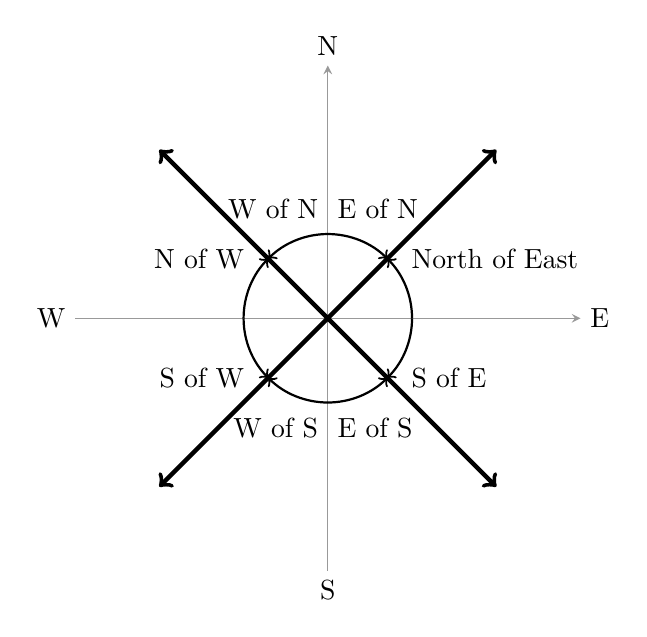
\begin{tikzpicture}
\pgfplotsset{compat=1.11}
    \begin{axis}[width=8cm, height=8cm,
        axis lines = middle,
        axis line style = {black!40},
        xlabel = E, x label style={anchor=west},
        ylabel = N, y label style={anchor=south},
        ymin=-3, ymax=3,
        xmin=-3, xmax=3,
        ticks=none,
        clip=false,
        ]
        \node[left] at (-3,0) {W};
        \node[below] at (0,-3) {S};
        \draw[ultra thick,<->] (-2,-2) -- (2,2);
        \draw[ultra thick,<->] (-2,2) -- (2,-2);
        \draw[thick,->] (1,0) arc (0:45:1) node[right=5pt] {North of East};
        \draw[thick,->] (0,1) arc (90:45:1);
        \draw[thick,->] (0,1) arc (90:135:1);
        \draw[thick,->] (-1,0) arc (180:135:1) node[left=5pt] {N of W};
        \draw[thick,->] (-1,0) arc (180:225:1) node[left=5pt] {S of W};
        \draw[thick,->] (0,-1) arc (270:225:1);
        \draw[thick,->] (0,-1) arc (270:315:1);
        \draw[thick,->] (1,0) arc (0:-45:1) node[right=5pt] {S of E};
        \node[right] at (0,1.3) {E of N};
        \node[left] at (0,1.3) {W of N};
        \node[left] at (0,-1.3) {W of S};
        \node[right] at (0,-1.3) {E of S};
    \end{axis}
\end{tikzpicture}
\end{minipage}%
\hspace{2em}
\begin{minipage}{0.5\textwidth}
\centering
    \begin{tabular}{c|c}
        \textbf{DO NOT USE} & \textbf{USE} \\
        \hline
        E of N & North of East\\
        W of N & N of W\\
        W of S & S of W\\
        E of S & S of E\\
    \end{tabular}
\end{minipage}

Two angles in the same quadrant are complimentary: they add up to \SI{90}{\degree}. For example, an \textbf{east of north} (E of N) angle is complementary to a \textbf{north of east} (N of E) angle. To convert degrees E of N to degrees N of E, calculate 90 minus the E of N angle. The same applies to other directions (e.g., W of S $\rightarrow$ S of W).

\subsection{Calculating Components Analytically}

Cosine (cos) and sine (sin) are trig functions on a calculator.

Cosine (cos) says, ``You give me the magnitude and direction (angle) of a vector; I give you the $x$-component.''.

Sine (cos) says, ``You give me the magnitude and direction (angle) of a vector; I give you the $y$-component.''

\begin{example}
    Vector $\vec{A}$ has a magnitude of 25 and is directed \SI{30}{\degree} north of east. (a) What is the $x$-component ($A_x$) of the vector? (b) What is the vector's $y$-component ($A_y$)?
\end{example}

\Solution Always sketch a picture to visualize the problem.

\begin{figure}[h!]
    \centering
\def\A{5}
\def\angle{30}
\begin{tikzpicture}
\pgfplotsset{compat=1.11}
\begin{axis}[width=8cm,height=8cm,
    axis lines=middle,
    axis line style={black!20},
    xmin=-5,xmax=5,ymin=-5,ymax=5,
    axis equal,
    ticks = none,
    xlabel = E, x label style={anchor=west},
    ylabel = N, y label style={anchor=south},
        ticks=none,
        clip=false,
        ]
        \node[left] at (axis cs: -5,0) {W};
        \node[below] at (axis cs: 0,-5) {S};
        \draw[thick] (axis cs: 1,0) arc (0:\angle:1);
        \node at (axis cs: 2,0.5) {\SI{\angle}{\degree}};
        \draw[ultra thick,black,->] (axis cs: 0,0) -- ++(axis direction cs: {\A*cos(\angle)},{\A*sin(\angle)}) node[right,align=left] {$\vec{A}=25$};
    \end{axis}
\end{tikzpicture}
\end{figure}

\textbf{Key idea}: The $x$-component ($A_x$) is equal to the magnitude of vector $\vec{A}$ multiplied by cosine (cos) of the angle from the $+x$-axis to the vector:

\begin{equation*}
    \vec{A}_x = 25 \cos{(\SI{30}{\degree})} = +21.65
\end{equation*}

(b) Likewise, the $y$-component ($A_y$) is equal to the magnitude of vector $\vec{A}$ multiplied by sine (sin) of the angle from the $+x$-axis to the vector:

\begin{equation*}
    \vec{A}_y = 25 \sin{(\SI{30}{\degree})} = +12.5
\end{equation*}

\textbf{Note}: Your calculator must be in ``degrees'' mode for these calculations to work.

\begin{example}
    Vector $\vec{A}$ has a magnitude of 49 at \SI{73}{\degree} north of west. Find the $x$- and $y$-components of $\vec{A}$.
\end{example}

\Solution The picture is

\begin{figure}[h!]
    \centering
\def\A{6}
\def\angle{73}
\begin{tikzpicture}
\pgfplotsset{compat=1.11}
\begin{axis}[width=8cm,height=8cm,
    axis lines=middle,
    axis line style={black!20},
    xmin=-6,xmax=6,ymin=-6,ymax=6,
    axis equal,
    ticks = none,
    xlabel = E, x label style={anchor=west},
    ylabel = N, y label style={anchor=south},
        ticks=none,
        clip=false,
        ]
        \node[left] at (-6,0) {W};
        \node[below] at (0,-6) {S};
        \draw[thick] (-1,0) arc (180:180-\angle:1);
        \node at (-1.1,1) {\SI{\angle}{\degree}};
        \draw[ultra thick,black,->] (0,0) -- ({-\A*cos(\angle)},{\A*sin(\angle)}) node[above] {$\vec{A} = 49$};
        \draw[dashed,thick,->] (0,0) -- ({-\A*cos(\angle)},0) node[below] {$\vec{A}_x$}; 
        \draw[dashed,thick,->] ({-\A*cos(\angle)},0) -- ({-\A*cos(\angle)},{\A*sin(\angle)}) node[below left] {$\vec{A}_y$}; 
    \end{axis}
\end{tikzpicture}%
\hspace{2em}
\begin{tikzpicture}
\pgfplotsset{compat=1.11}
\begin{axis}[width=8cm,height=8cm,
    axis lines=middle,
    axis line style={black!20},
    xmin=-6,xmax=6,ymin=-6,ymax=6,
    % axis equal,
    ticks = none,
    xlabel = E, x label style={anchor=west},
    ylabel = N, y label style={anchor=south},
        ticks=none,
        clip=false,
        ]
        \node[left] at (-6,0) {W};
        \node[below] at (0,-6) {S};
        \draw[thick] (-1,0) arc (180:180-\angle:1);
        \draw[thick,red] (1,0) arc (0:180-\angle:1);
        \node[red] at (0.7,1.4) {$\beta$};
        \node at (-1.5,0.8) {\SI{\angle}{\degree}};
        \draw[ultra thick,black,->] (0,0) -- ({-\A*cos(\angle)},{\A*sin(\angle)}) node[left] {$\vec{A} = 49$};
    \end{axis}
\end{tikzpicture}
\end{figure}

The given angle, \SI{73}{\degree}, is measured from the $-x$ axis, so it's not in standard position; its application calculates only the \textit{magnitude} (not direction) of $x$- and $y$-components: 


\begin{align*}
    A_x &= 49 \cos{(73)} = 14.3\\[1ex]
    A_y &= 49 \sin{(73)} = 46.9
\end{align*}


Directions are inferred by noting that the $x$-component vector points left, towards the $-x$ axis, making $A_x$ negative, and that the $y$-component vector, pointing towards $+y$, is positive:

\begin{equation*}
    \vec{A}_x = -14.3\ , \hspace{1em}
    \vec{A}_y = +46.9
\end{equation*}

An alternative solution: Only angles in standard position yield both magnitude and direction. Here, the \href{https://mathworld.wolfram.com/SupplementaryAngles.html}{supplementary angle} of \SI{73}{\degree} ($\beta$ in the figure) \textit{is} in standard position and is found by

\begin{equation*}
    \beta = 180 - 73 = \SI{107}{\degree}
\end{equation*}

The vector components are

\begin{align*}
    \vec{A}_x &= 49 \cos{(107)} = -14.3\\[1ex]
    \vec{A}_y &= 49 \sin{(107)} = +46.9
\end{align*}

\hrule

\begin{example}
    Hedwig the Owl starts at his nest and undergoes a displacement of 12 kilometers at \SI{32}{\degree} east of north. (a) What is the $x$-component (East) of his displacement? (b) What is the $y$-component (North)?
\end{example}

\Solution

\begin{figure}[h!]
    \centering
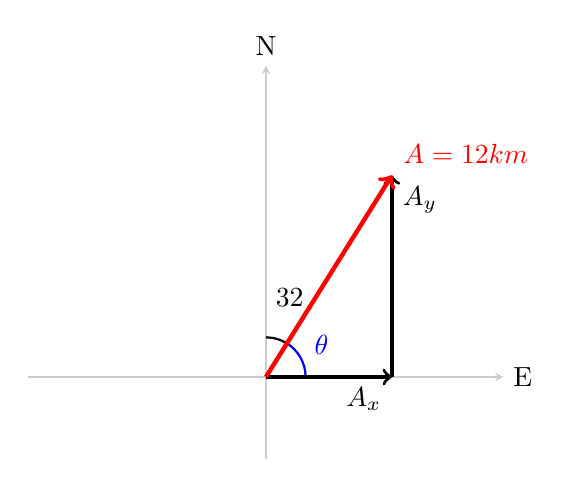
\begin{tikzpicture}
\def\A{3}
\def\angle{58}
\pgfplotsset{compat=1.11}
\begin{axis}[width=3in,
    axis lines=middle,
    xmin=-3,xmax=3,ymin=-0.1,ymax=3,
    axis equal,
    ticks = none,
    xlabel = E, x label style={anchor=west},
    ylabel = N, y label style={anchor=south},
    axis line style={black!20},
    clip=false,
    ]
    \draw[thick,blue] (0.5,0) arc (0:\angle:0.5);
    \node[blue] at (0.7,0.4) {$\theta$};
    \draw[->,very thick] (0,0) -- ({\A*cos(\angle)},0) node[below left] {$A_x$};
    \draw[->,very thick] ({\A*cos(\angle)},0) -- ({\A*cos(\angle)},{\A*sin(\angle)}) node[below right] {$A_y$};
    \draw[thick] (0,0.5) arc (90:58:0.5);
    \node at (0.3,1) {\SI{32}{\degree}};
    \draw[->,ultra thick,red] (0,0) -- ({\A*cos(\angle)},{\A*sin(\angle)}) node[above right] {$A=\SI{12}{km}$};
\end{axis}
\end{tikzpicture}
\end{figure}

Do not use the E of N angle of \SI{32}{\degree}. Convert it to N of E as follows:

\begin{equation*}
    \theta = \SI{90}{\degree} - \SI{32}{\degree} = \SI{58}{\degree}
\end{equation*}

The angle $\theta = \SI{58}{\degree}$, which is in standard position, may now be used in our $\cos$ and $\sin$ functions.

(a) The $x$-component equals the magnitude of the vector times the cosine of the angle:

\begin{equation*}
    \vec{A}_x = 12 \cos{(58)} = +\SI{6.36}{km}
\end{equation*}

(b) The $y$-component is

\begin{equation*}
    \vec{A}_y = 12 \sin{(58)} = +\SI{10.18}{km}
\end{equation*}

\hrule

\begin{example}
    The Eiffel Tower is \SI{789}{ft} and \SI{114}{\degree} from Jarred the tourist. (a) How far north is the Eiffel tower? (b) How far west?
\end{example}

\Solution

\begin{figure}[h!]
    \centering
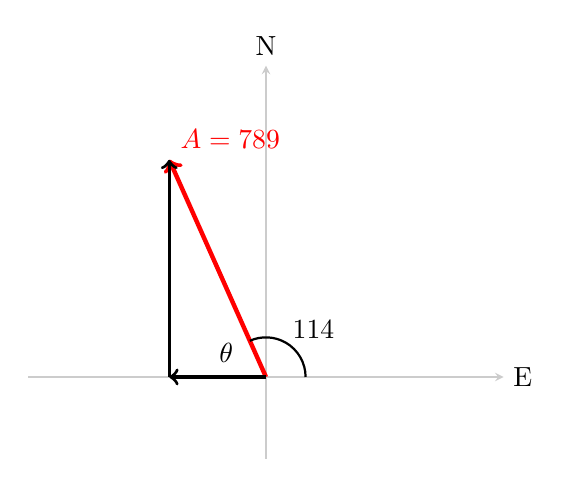
\begin{tikzpicture}
\def\A{3}
\def\angle{114}
\pgfplotsset{compat=1.11}
\begin{axis}[width=3in,
    axis lines=middle,
    xmin=-3,xmax=3,ymin=-0.1,ymax=3,
    axis equal,
    ticks = none,
    xlabel = E, x label style={anchor=west},
    ylabel = N, y label style={anchor=south},
    axis line style={black!20},
    ]
    \draw[->,ultra thick,red] (0,0) -- ({\A*cos(\angle)},{\A*sin(\angle)}) node[above right] {$A=789$};
    \draw[thick] (0.5,0) arc (0:\angle:0.5);
    \node at (0.6,0.6) {\SI{114}{\degree}};
    \draw[->,very thick] (0,0) -- ({\A*cos(\angle)},0);
    \draw[->,very thick] ({\A*cos(\angle)},0) -- ({\A*cos(\angle)},{\A*sin(\angle)});
    \node at (-0.5,0.3) {$\theta$};
\end{axis}
\end{tikzpicture}
\end{figure}

The angle $\theta$ is

\begin{equation*}
    \theta = \SI{180}{\degree} - \SI{114}{\degree} = \SI{66}{\degree}
\end{equation*}

(a) The magnitude of the $x$-component is 

\begin{equation*}
    A_x = 789 \cos{(66)} = \SI{320.9}{ft}
\end{equation*}

Therefore, the Eiffel Tower is \SI{320.9}{ft} west.

(b) The magnitude of the $y$-component is

\begin{equation*}
    A_y = 789 \sin{(66)} = \SI{720.8}{ft}
\end{equation*}

Therefore, it's \SI{720.8}{ft} north.

An alternative solution: The standard position angle $\SI{114}{\degree}$ directly yields 

\begin{align*}
    \vec{A}_x &= 789 \cos{(114)} = -\SI{320.9}{ft}\\[1ex]
    \vec{A}_y &= 789 \sin{(114)} = +\SI{720.8}{ft}
\end{align*}

\begin{example}
    Pac-Man takes 3 steps to the right and 4 steps up. (a) What is the magnitude of his resultant displacement vector? (b) What is the direction of the resultant vector?
\end{example}

\Solution The picture is

\begin{figure}[h!]
    \centering
\begin{tikzpicture}
\def\A{7}
\def\angle{53.13}
\pgfplotsset{compat=1.11}
\begin{axis}[width=8cm,
    axis lines=middle,
    xmin=-1,xmax=7,ymin=-1,ymax=7,
    axis equal,
    ticks = none,
    xlabel = E, x label style={anchor=west},
    ylabel = N, y label style={anchor=south},
    axis line style={black!20},
    clip=false,
    ] 
    \draw[thick,->] (0,0) -- ({\A*cos(\angle)},0) node[below] {$\vec{A}_x = 3$};
    \draw[thick,->] ({\A*cos(\angle)},0) -- ++(axis direction cs: 0,{\A*sin(\angle)}) node[right] {$\vec{A}_y = 4$};
    \draw[ultra thick,->,red] (0,0) -- ({\A*cos(\angle)},{\A*sin(\angle)}) node[above left] {$\vec{A}$};
    \draw[thick] (1,0) arc (0:\angle:1);
    \node at (1.3,0.6) {$\theta$};
    \end{axis}
\end{tikzpicture}
\end{figure}

(a) The \href{https://mathworld.wolfram.com/PythagoreanTheorem.html}{Pythagorean theorem} ($a^2 + b^2 = c^2$) relates the three sides of a right triangle. Since vector $\vec{A}$ and its components form a right triangle, it follows that the magnitude of $\vec{A}$ is given by

\begin{equation*}
    3^2 + 4^2 = A^2
\end{equation*}

To solve for $A$, the magnitude of the vector, take the square root of both sides:

\begin{equation*}
    A = \sqrt{3^2 + 4^2} = 5
\end{equation*}

(b) The direction, given by $\theta$, is found by taking the inverse tangent (another trig function) of the $y$-component divided by the $x$-component:

\begin{equation*}
    \theta = \tan^{-1}\left(\frac{4}{3}\right) = \SI{53.1}{\degree}
\end{equation*}

\hrule

\clearpage

\begin{mdframed}[backgroundcolor=black!10]
\textit{Vector summary}. In general, consider vector $\vec{A}$, of magnitude $A$, whose direction is given by an angle $\theta$ that is in standard position. The $x$- and $y$-components of $\vec{A}$, the magnitude of $\vec{A}$, and the directional angle $\theta$ are generally given by the following relations: 

\begin{equation*}
    \vec{A}_x = A \cos{\theta}\ , \hspace{1em}
    \vec{A}_y = A \sin{\theta}\ , \hspace{1em}
    A = \sqrt{A_x^2 + A_y^2}\ , \hspace{1em}
    \theta = \tan^{-1}\left(\frac{A_y}{A_x}\right)
\end{equation*}
\end{mdframed}

\begin{figure}[h!]
    \centering
    \pgfplotsset{compat=1.11}
    \def\A{6}
    \def\angle{55}
\begin{tikzpicture}
    \begin{axis}[width=8cm,height=8cm,
        axis lines=middle,
        axis line style={black!20},
        xmin=-6,xmax=6,
        ymin=-6,ymax=6,
        clip=false,
        ticks=none,
        xlabel=$+x$,
        x label style={anchor=west},
        ylabel=$+y$, y label style={anchor=south},
    ]
    \draw[thick,->] (0,0) -- ({\A*cos(\angle)},0) node[below] {$\vec{A}_x$};
    \draw[thick,->] ({\A*cos(\angle)},0) -- ({\A*cos(\angle)},{\A*sin(\angle)}) node[below right] {$\vec{A}_y$};
    \draw[ultra thick,red,->] (0,0) -- ({\A*cos(\angle)},{\A*sin(\angle)}) node[above,red] {$\vec{A}$};
    \draw[thick] (1,0) arc (0:\angle:1); 
    \node at (1.3,0.7) {$\theta$};
    \end{axis}
\end{tikzpicture}
\end{figure}

\begin{example}
    Alice undergoes two displacements: 49 meters east and 67 meters north. Her third displacement gets her back to the initial position. (a) What is the magnitude of the resultant (3rd) displacement vector? (b) What is the direction as measured from \SI{0}{\degree} (i.e., from $+x$ or East)?
\end{example}

\Solution It's helpful to draw two pictures. The first shows the $x$- and $y$ components and the resultant vector $R$ that leads back to the origin.

\begin{figure}[h!]
    \centering
\begin{tikzpicture}
\def\A{3}
\def\angle{53.82}
\pgfplotsset{compat=1.11}
\begin{axis}[width=8cm,
    axis lines=middle,
    xmin=-3,xmax=3,ymin=-3,ymax=3,
    axis equal,
    ticks = none,
    xlabel = E, x label style={anchor=west},
    ylabel = N, y label style={anchor=south},
    axis line style={black!20},
    clip=false
    ]
    \draw[->,ultra thick,red]  ({\A*cos(\angle)},{\A*sin(\angle)}) -- (0,0);
    \node[red] at (0.3,0.9) {$R$};
    \draw[thick] (0.7,0) arc (0:\angle:0.7);
    \node at (0.9,0.35) {$\alpha$};
    \draw[->,very thick] (0,0) -- ({\A*cos(\angle)},0) node[below] {\SI{49}{m}};
    \draw[->,very thick] ({\A*cos(\angle)},0) -- ({\A*cos(\angle)},{\A*sin(\angle)}) node[right] {\SI{67}{m}};
\end{axis}
\end{tikzpicture}%
\hfill
\begin{tikzpicture}
\def\A{3}
\def\angle{53.82}
\pgfplotsset{compat=1.11}
\begin{axis}[width=8cm,
    axis lines=middle,
    xmin=-3,xmax=3,ymin=-3,ymax=3,
    axis equal,
    ticks = none,
    xlabel = E, x label style={anchor=west},
    ylabel = N, y label style={anchor=south},
    axis line style={black!20},
    clip=false
    ]
    \begin{scope}[xshift=-1.57cm,yshift=-2.13cm]
    \draw[->,ultra thick,red] ({\A*cos(\angle)},{\A*sin(\angle)}) -- (0,0);
    \node[red] at (0.3,-0.3) {$R$};
    \draw[dashed] (0,0) -- (1.2,0);
    \draw[thick] (0.6,0) arc (0:\angle:0.6);
    \node at (0.8,0.35) {$\alpha$};
    \end{scope}
    \draw[thick] (-0.5,0) arc (180:180+\angle:0.5);
    \node at (-0.65,-0.3) {$\alpha$};
    \draw[thick,blue,->] (1,0) arc (0:180+\angle:1);
    \node[blue] at (-0.5,1.2) {$\theta$};
\end{axis}
\end{tikzpicture}
\end{figure}

The magnitude of the resultant is

\begin{equation*}
    R = \sqrt{49^2 + 67^2} = \SI{83}{m}
\end{equation*}

(b) Angle $\alpha$, while \textit{not} the desired angle, is necessary to find direction and is calculated as

\begin{equation*}
    \alpha = \tan^{-1}\left(\frac{67}{49}\right) = \SI{53.8}{\degree}
\end{equation*}

In the second picture, vector $\vec{R}$ is re-centered at standard position. Since $\vec{R}$ is in quadrant III, it's direction ($\theta$) is \SI{180}{\degree} (from quadrants I and II) plus $\alpha$:

\begin{equation*}
    \theta = 180 + \alpha = 180 + 53.8 = \SI{233.8}{\degree}\ .
\end{equation*}


\subsection{Horizontally Launched Projectiles}

\begin{figure}[h!]
    \centering
    \begin{tabular}{cl|cl}
    \hline
    \textbf{Symbol} & \textbf{Quantity} & \textbf{Unit} & \textbf{Unit Symbol}  \\
    \hline\hline
        $d_x$ & horizontal displacement (or position) & meter & m\\
        $d_y$ & vertical displacement (or position) & meter & m\\
        $t$ & time & second & s\\
        $v$ & velocity & meter per second & m/s\\
        $v_0$ & initial velocity & meter per second & m/s\\
        $v_{0y}$ & vertical component of initial velocity & meter per second & m/s\\
        $v_{0x}$ & horizontal component of initial velocity & meter per second & m/s\\
        $v_y$ & vertical velocity & meter per second & m/s\\
        $v_x$ & horizontal velocity & meter per second & m/s\\
        $a_y$ & vertical component of acceleration & meter per second squared & $\SI{}{m/s^2}$\\
        $g$ & acceleration due to gravity & meter per second squared & \SI{}{m/s^2}\\
        % $\theta$ & projectile \textbf{instantaneous} angle & degrees & \SI{}{\degree}\\
        % $\theta_0$ & projectile \textbf{launch} angle & degrees & \SI{}{\degree}\\
        % $y_{\mathrm{max}}$ & maximum projectile height & meter & m\\
        % $t_{\mathrm{max}}$ & time from launch to $y_{\mathrm{max}}$ & second & s\\
        % $R$ & projectile range & meter & m\\
    \hline
    \end{tabular}
    % \caption*{Symbols and units of physical quantities in projectile motion. As you read the information below, refer back to this table frequently to review what a symbol means.}
    \label{fig:my_label}
\end{figure}

Projectile motion is the motion of an object thrown into the air. The object,known as the ``projectile,'' experiences only downward acceleration due to gravity. The trajectory is the curved path of a projectile through the air. In projectile motion, horizontal and vertical motions (e.g., displacement, velocity, acceleration) are independent: their $x$- and $y$-components don't influence each other. For example, a projectile's $\vec{v}_x$ vector can be analyzed separately from its $\vec{v}_y$.

A \textit{horizontally launched projectile} is an object that is thrown with an initial velocity that is entirely horizontal. In such a case, the $y$-component of the initial velocity is zero, and the $x$-component of initial velocity is the velocity at which the object is launched. 

\begin{mdframed}[backgroundcolor=black!10]
The horizontal motion of a horizontally launched projectile is governed by these equations:
\vspace{-1em}

\begin{align*}
    \vec{a}_x &= 0\\[0.5ex]
    \vec{v}_x &= \mathrm{constant} = \vec{v}_{0x}\\[0.5ex]
    \vec{d}_x &= \vec{v}_{0x} \cdot t\\[0.5ex]
\end{align*}
\vspace{-3em}

\begin{center}
        \begin{tabular}{cl|cl}
    \hline
    \textbf{Symbol} & \textbf{Quantity} & \textbf{Unit} & \textbf{Unit Symbol}  \\
    \hline\hline
        $a_x$ & horizontal component of acceleration & meter per second squared & $\SI{}{m/s^2}$\\
        $v_x$ & horizontal velocity & meter per second & m/s\\
        $v_{0x}$ & horizontal component of initial velocity & meter per second & m/s\\
        $d_x$ & horizontal displacement (or position) & meter & m\\
        $t$ & time & second & s\\
    \hline
    \end{tabular}
\end{center}
% \textbf{Note}: The velocity at which the projectile is launched is the same as $\vec{v}_{0x}$.
\end{mdframed}

\begin{mdframed}[backgroundcolor=black!10]
After launch, the projectile accelerates downward due to gravity. The magnitude of this acceleration is

\begin{equation*}
    g = \SI{9.8}{m/s^2}\ .
\end{equation*}
\end{mdframed}

\begin{mdframed}[backgroundcolor=black!10]
The \textit{vertical} motion of a horizontally launched projectile is governed by these equations:
\vspace{-1em}

\begin{align*}
    \vec{a}_y &= -g = -\SI{9.8}{m/s^2}\\
    \vec{v}_y &= - gt\\
    \vec{d}_y &= -\frac{1}{2} g t^2\\
\end{align*}
\vspace{-3em}

\begin{center}
    \begin{tabular}{cl|cl}
    \hline
    \textbf{Symbol} & \textbf{Quantity} & \textbf{Unit} & \textbf{Unit Symbol}  \\
    \hline\hline
        $a_y$ & vertical component of acceleration & meter per second squared & $\SI{}{m/s^2}$\\
        $v_y$ & vertical velocity & meter per second & m/s\\
        $v_{0y}$ & vertical component of initial velocity & meter per second & m/s\\
        $d_y$ & vertical displacement (or position) & meter & m\\
        $t$ & time & second & s\\
    \hline
    \end{tabular}
\end{center}
\end{mdframed}

% Range is

% \begin{equation*}
%     R = \frac{v^2_0 \sin{2\theta_0}}{g}\ .
% \end{equation*}

% The equation of the path is

% \begin{equation*}
%     y =  -\frac{g x^2}{2\left(v_0 \cos{\theta_0}\right)^2} + \left(\tan{\theta_0}\right) x + y_0
% \end{equation*}

\begin{example} \label{r4IUyp}
    A metallic ball is shot horizontally at \SI{12}{m/s} from the top of a tall cliff. (a) Calculate horizontal components of velocity at 1-second time intervals for the first 5 seconds of motion. (b) Do the same for vertical components.
\end{example}

\begin{figure}[h!]
    \centering
    \begin{tikzpicture} 
    \tikzmath{
        \gravity = 9.8;
        \vi = 28.6;
        \yi = 60;
        \thetai = 0.0;
        \ys = 1.3;
    }
    \pgfplotsset{compat=1.11}
        \begin{axis}[width=6cm,height=6cm,ticks=none,
        axis line style = {black!50},
        axis lines = middle,
        clip=false,
        ylabel style= {anchor=south},
        xlabel style= {anchor=west},
        ylabel = $y$,
        xlabel = $x$,
        xmin=0, xmax=120,
        ymin=0, ymax=80,
        ]
        \addplot [dashed,
            domain=0:100,
            samples=100, 
            color=black!50,
        ]
        {\yi + tan(\thetai)*x - \gravity*x^2/(2*(\vi*cos(\thetai))^2)}; %equation of path
        \fill (0,\yi) circle (2pt) node[left] {$y_0$};
        \draw[thick,->,red] (0,\yi) -- (12,\yi) node[above] {$v_x$};
        \fill (20,57.60) circle (2pt); %Calculated using equator of path
        \draw[thick,->,red] (20,57.60) -- ++(axis direction cs: 12,0) node[above] {$v_x$};
        \draw[thick,->,red] (20,57.60) -- ++(axis direction cs: 0,-5*\ys^0) node[left] {$v_y$};
        \fill (40,50.42) circle (2pt);
        \draw[thick,->,red] (40,50.42) -- ++(axis direction cs: 12,0) node[above] {$v_x$};
        \draw[thick,->,red] (40,50.42) -- ++(axis direction cs: 0,-5*\ys^1) node[left] {$v_y$};
        \fill (60,38.43) circle (2pt);
        \draw[thick,->,red] (60,38.43) -- ++(axis direction cs: 12,0) node[above] {$v_x$};
        \draw[thick,->,red] (60,38.43) -- ++(axis direction cs: 0,-5*\ys^2) node[left] {$v_y$};
        \fill (80,21.66) circle (2pt);
        \draw[thick,->,red] (80,21.66) -- ++(axis direction cs: 12,0) node[above] {$v_x$};
        \draw[thick,->,red] (80,21.66) -- ++(axis direction cs: 0,-5*\ys^3) node[left] {$v_y$};
        \fill ({\vi*sqrt(2*\yi/\gravity)},0) circle (2pt) node[below left] {$x_f$};
        \draw[thick,->,red] ({\vi*sqrt(2*\yi/\gravity)},0) -- ++(axis direction cs: 12,0) node[above] {$v_x$};
        \draw[thick,->,red] ({\vi*sqrt(2*\yi/\gravity)},0) -- ++(axis direction cs: 0,-5*\ys^4) node[left] {$v_y$};
        \end{axis}
    \end{tikzpicture}
\end{figure}

\Solution (a) We are given initial velocity: $v_0 = \SI{12}{m/s}$. Since $v_0$ is entirely horizontal, the $x$-component of $v_0$ is also \SI{12}{m/s}:

\begin{equation*}
    \vec{v}_{0x} = +\SI{12}{m/s}
\end{equation*}

For horizontal motion, acceleration is zero:

\begin{equation*}
    a_x = 0\ .
\end{equation*}

Zero horizontal acceleration implies no change in horizontal velocity:
\vspace{-1em}

\begin{align*}
    v_x \text{ at \SI{1.0}{s}} &= \SI{12}{m/s}\\[0.5ex]
    v_x \text{ at \SI{2.0}{s}} &= \SI{12}{m/s}\\[0.5ex]
    v_x \text{ at \SI{3.0}{s}} &= \SI{12}{m/s}\\[0.5ex]
    v_x \text{ at \SI{4.0}{s}} &= \SI{12}{m/s}\\[0.5ex]
    v_x \text{ at \SI{5.0}{s}} &= \SI{12}{m/s}\\[0.5ex]
\end{align*}

(b) Recall that the magnitude of acceleration due to gravity is $g = \SI{9.8}{m/s^2}$. The vertical component of velocity for a horizontally launched projectile is 

\begin{equation*} 
    v_y = -g t = -9.8 t
\end{equation*}

Therefore, vertical velocities are

\begin{align*}
    v_y \text{ at \SI{1.0}{s}} &= (-9.8)(1) = \SI{-9.8}{m/s}\\[0.5ex]
    v_y \text{ at \SI{2.0}{s}} &= (-9.8)(2) = \SI{-19.6}{m/s}\\[0.5ex]
    v_y \text{ at \SI{3.0}{s}} &= (-9.8)(3) = \SI{-29.4}{m/s}\\[0.5ex]
    v_y \text{ at \SI{4.0}{s}} &= (-9.8)(4) = \SI{-39.2}{m/s}\\[0.5ex]
    v_y \text{ at \SI{5.0}{s}} &= (-9.8)(5) = \SI{-49.0}{m/s}\\[0.5ex]
\end{align*}

\begin{example}
    For the projectile in Example~\ref{r4IUyp}, (a) calculate horizontal components of displacement at 1-second time intervals for 5 seconds. (b) Do the same for vertical components of displacement.
\end{example}

\begin{figure}[h!]
    \centering
    \begin{tikzpicture} 
    \tikzmath{
        \gravity = 9.8;
        \vi = 28.6;
        \yi = 60;
        \thetai = 0.0;
        \ys = 1.3;
        \x1 = 20; \y1 = 57.60;
        \x2 = 40; \y2 = 50.42;
        \x3 = 60; \y3 = 38.43;
        \x4 = 80; \y4 = 21.66;
        \x5 = \vi*sqrt(2*\yi/\gravity); \y5 = 0;
    }
    \pgfplotsset{compat=1.11}
        \begin{axis}[width=8cm,height=8cm,ticks=none,
        axis line style = {black!50},
        axis lines = middle,
        clip=false,
        ylabel style= {anchor=south},
        xlabel style= {anchor=west},
        ylabel = $y$,
        xlabel = $x$,
        xmin=0, xmax=120,
        ymin=0, ymax=80,
        ]
        \addplot [dashed,
            domain=0:100,
            samples=100, 
            color=black!50,
        ]
        {\yi + tan(\thetai)*x - \gravity*x^2/(2*(\vi*cos(\thetai))^2)}; %equation of path
        \fill (0,\yi) circle (3pt) node[left] {$y_0$};
        \fill (\x1,\y1) circle (3pt); %Calculated using equator of path
        \draw[->,thick,red!80,dashed] (0,\y1) -- ++(axis direction cs: \x1,0) node[below left] {$d_x$};
        \draw[->,red] (\x1,\yi) -- ++(axis direction cs: 0,\y1-\yi) node[above right] {$d_y$};
        \fill (\x2,\y2) circle (3pt);
        \draw[->,thick,red!80,dashed] (0,\y2) -- ++(axis direction cs: \x2,0) node[below left] {$d_x$};
        \draw[->,thick,red!80,dashed] (\x2,\yi) -- ++(axis direction cs: 0,\y2-\yi) node[above right] {$d_y$};
        \fill (\x3,\y3) circle (3pt);
        \draw[->,thick,red!80,dashed] (0,\y3) -- ++(axis direction cs: \x3,0) node[below left] {$d_x$};
        \draw[->,thick,red!80,dashed] (\x3,\yi) -- ++(axis direction cs: 0,\y3-\yi) node[above right] {$d_y$};
        \fill (\x4,\y4) circle (3pt);
        \draw[->,thick,red!80,dashed] (0,\y4) -- ++(axis direction cs: \x4,0) node[below left] {$d_x$};
        \draw[->,thick,red!80,dashed] (\x4,\yi) -- ++(axis direction cs: 0,\y4-\yi) node[above right] {$d_y$};
        \fill (\x5,\y5) circle (3pt);
        \draw[->,thick,red!80,dashed] (0,\y5) -- ++(axis direction cs: \x5,0) node[below left] {$d_x$};
        \draw[->,thick,red!80,dashed] (\x5,\yi) -- ++(axis direction cs: 0,\y5-\yi) node[above right] {$d_y$};
        \end{axis}
    \end{tikzpicture}
\end{figure}

\Solution (a) Initial velocity is

\begin{equation*}
    v_0 = v_{0x} = \SI{12}{m/s}
\end{equation*}

Horizontal displacement is given by

\begin{equation*}
    d_x = v_{0x} \cdot t
\end{equation*}

The components are

\begin{align*}
    d_x \text{ at \SI{1.0}{s}} &= (\SI{12}{m/s})(\SI{1.0}{s}) = \SI{12}{m}\\[0.5ex]
    d_x \text{ at \SI{2.0}{s}} &= (\SI{12}{m/s})(\SI{2.0}{s}) = \SI{24}{m}\\[0.5ex]
    d_x \text{ at \SI{3.0}{s}} &= (\SI{12}{m/s})(\SI{3.0}{s}) = \SI{36}{m}\\[0.5ex]
    d_x \text{ at \SI{4.0}{s}} &= (\SI{12}{m/s})(\SI{4.0}{s}) = \SI{48}{m}\\[0.5ex]
    d_x \text{ at \SI{5.0}{s}} &= (\SI{12}{m/s})(\SI{5.0}{s}) = \SI{60}{m}\\[0.5ex]
\end{align*}

(b) Recalling that $g=\SI{9.8}{m/s^2}$,  the vertical displacement is given by

\begin{equation*}
    d_y = -\frac{1}{2} g t^2 = -\frac{1}{2}(9.8) t^2 = -4.9 t^2
\end{equation*}

Vertical displacements are
\vspace{-2em}

\begin{align*}
    d_y \text{ at \SI{1.0}{s}} &= -(4.9)(1^2) = -\SI{4.9}{m}\\[0.5ex]
    d_y \text{ at \SI{2.0}{s}} &= -(4.9)(2^2) = -\SI{19.6}{m}\\[0.5ex]
    d_y \text{ at \SI{3.0}{s}} &= -(4.9)(3^2) = -\SI{44.1}{m}\\[0.5ex]
    d_y \text{ at \SI{4.0}{s}} &= -(4.9)(4^2) = -\SI{78.4}{m}\\[0.5ex]
    d_y \text{ at \SI{5.0}{s}} &= -(4.9)(5^2) = -\SI{122.5}{m}\\[0.5ex]
\end{align*}
\vspace{-1em}

\begin{example} \label{i3PZ3N}
    Pel\'{e} kicks a soccer ball horizontally at a speed of \SI{30}{m/s} from the top of a building that is 500 meters tall. How long does the ball take to impact the ground?
\end{example}

\begin{figure}[h!]
    \centering
    \begin{tikzpicture} 
    \tikzmath{
        \gravity = 9.8;
        \vi = 28.6;
        \yi = 60;
        \thetai = 0.0;
        \ys = 1.3;
        \x1 = 20; \y1 = 57.60;
        \x2 = 40; \y2 = 50.42;
        \x3 = 60; \y3 = 38.43;
        \x4 = 80; \y4 = 21.66;
        \x5 = \vi*sqrt(2*\yi/\gravity); \y5 = 0;
    }
    \pgfplotsset{compat=1.11}
        \begin{axis}[width=6cm,height=6cm,ticks=none,
        axis line style = {black!50},
        axis lines = middle,
        clip=false,
        ylabel style= {anchor=south},
        xlabel style= {anchor=west},
        ylabel = $y$,
        xlabel = $x$,
        xmin=0, xmax=120,
        ymin=0, ymax=80,
        ]
        \addplot [dashed,
            domain=0:100,
            samples=100, 
            color=black!50,
        ]
        {\yi + tan(\thetai)*x - \gravity*x^2/(2*(\vi*cos(\thetai))^2)}; %equation of path
        \fill (0,\yi) circle (2pt);% node[left] {$y_0$};
        \fill (\x1,\y1) circle (2pt); %Calculated using equator of path
        \fill (\x2,\y2) circle (2pt);
        \fill (\x3,\y3) circle (2pt);
        \fill (\x4,\y4) circle (2pt);
        \fill (\x5,\y5) circle (2pt);
        \end{axis}
    \end{tikzpicture}
\end{figure}

\Solution The impact time depends on the height from which the ball drops. This height is the magnitude of the ball's vertical displacement ($d_y$):

\begin{equation*}
    d_y = -\frac{1}{2} g t^2\ \hspace{2em} (\text{where } g = \SI{9.8}{m/s^2})\ .
\end{equation*}

The ball drops 500 meters, so it's vertical displacement is $d_y = \SI{-500}{m}$. Plugging in values into the equation above leads to

\begin{equation*}
    -500 = -\frac{1}{2} (9.8) t^2 = -4.9 t^2\ ,
\end{equation*}

or, eliminating the negative signs,

\begin{equation*}
    500 = 4.9 t^2\ .
\end{equation*}

To find impact time, we solve this equation for time $t$ as follows:

\begin{align*}
    % \hspace{-10em} \textbf{Multiply $\frac{1}{2}$ by 9.8} 
    % \hspace{5em} & 500 = \frac{1}{2} (9.8) t^2\\[1ex] 
    % \hspace{-10em} \textbf{Simplify} \hspace{5em} & 500 = 4.9 t^2\\[1ex] 
   \hspace{-10em} \textbf{Divide by $4.9$} \hspace{5em} & \frac{500}{\textcolor{red}{4.9}} = \frac{\cancel{4.9}\,t^2}{\textcolor{red}{\cancel{4.9}}}\\[1ex] 
    \hspace{-10em} \textbf{Simplify} \hspace{5em} & 102 = t^2\\[1ex] 
    \hspace{-10em} \textbf{Put $t$ on the left} \hspace{5em} & t^2 = 102\\[1ex] 
    \hspace{-10em} \textbf{Take square root} \hspace{5em} & \sqrt{t^2} = \sqrt{102} = 10.1\\[1ex] 
\end{align*}

Therefore, the time the ball will take to impact the floor is

\begin{equation*}
    t = \SI{10.1}{s}\ .
\end{equation*}

\begin{example}
   For the ball in Example~\ref{i3PZ3N}, what is the magnitude of the velocity the instant the ball impacts the ground? This is known as the ``entry speed.'' 
\end{example}

\begin{figure}[h!]
    \centering
    \begin{tikzpicture} 
    \tikzmath{
        \gravity = 9.8;
        \vi = 28.6;
        \yi = 60;
        \thetai = 0.0;
        \ys = 1.3;
    }
    \pgfplotsset{compat=1.11}
        \begin{axis}[width=8cm,height=8cm,ticks=none,
        axis line style = {black!20},
        axis lines = middle,
        clip=false,
        ylabel style= {anchor=south},
        xlabel style= {anchor=west},
        ylabel = $y$,
        xlabel = $x$,
        xmin=0, xmax=120,
        ymin=-80, ymax=80,
        ]
        \addplot [dashed,
            domain=0:100,
            samples=100, 
            color=black!50,
        ]
        {\yi + tan(\thetai)*x - \gravity*x^2/(2*(\vi*cos(\thetai))^2)}; %equation of path
        \fill (0,\yi) circle (2pt) node[left] {$t=0$};
        % \draw[thick,->,red] (0,\yi) -- (12,\yi) node[above] {$v_x$};
        % \fill (20,57.60) circle (2pt); %Calculated using equator of path
        % \draw[thick,->,red] (20,57.60) -- ++(axis direction cs: 12,0) node[above] {$v_x$};
        % \draw[thick,->,red] (20,57.60) -- ++(axis direction cs: 0,-5*\ys^0) node[left] {$v_y$};
        % \fill (40,50.42) circle (2pt);
        % \draw[thick,->,red] (40,50.42) -- ++(axis direction cs: 12,0) node[above] {$v_x$};
        % \draw[thick,->,red] (40,50.42) -- ++(axis direction cs: 0,-5*\ys^1) node[left] {$v_y$};
        % \fill (60,38.43) circle (2pt);
        % \draw[thick,->,red] (60,38.43) -- ++(axis direction cs: 12,0) node[above] {$v_x$};
        % \draw[thick,->,red] (60,38.43) -- ++(axis direction cs: 0,-5*\ys^2) node[left] {$v_y$};
        % \fill (80,21.66) circle (2pt);
        % \draw[thick,->,red] (80,21.66) -- ++(axis direction cs: 12,0) node[above] {$v_x$};
        % \draw[thick,->,red] (80,21.66) -- ++(axis direction cs: 0,-5*\ys^3) node[left] {$v_y$};
        \fill ({\vi*sqrt(2*\yi/\gravity)},0) circle (2pt) node[below left=5pt,align=left] {impact\\ $t=10.1$};
        \draw[thick,->,red] ({\vi*sqrt(2*\yi/\gravity)},0) -- ++(axis direction cs: 12,0) node[above] {$v_x$};
        \draw[thick,->,red] ({\vi*sqrt(2*\yi/\gravity)},0) -- ++(axis direction cs: 0,-40) node[left] {$v_y$};
        \end{axis}
    \end{tikzpicture}
\end{figure}

\Solution The horizontal velocity at impact is the same as its initial value:

\begin{equation*}
    v_x = v_{0x} = +\SI{30}{m/s}
\end{equation*}

As calculated in the previous example, impact occurs at time $t=\SI{10.1}{s}$, so the vertical component of velocity at impact is

\begin{equation*}
    v_y = - g t =  - (9.8)(10.1) = \SI{-98.99}{m/s}\ .
\end{equation*}

By the Pythagorean Theorem (see ``Vectors'' section above), the magnitude of velocity at impact is

\begin{equation*}
    v = \sqrt{v_x^2 + v_y^2}
    = \sqrt{\left(30\right)^2 + \left(-98.99\right)^2}
    = \SI{103.4}{m/s}
\end{equation*}

This is the entry speed.


\end{document}



% Learning Goals:
% \vspace{-1em}
% \begin{enumerate}
%     \setlength\itemsep{0.1ex}
%     \item Identify the $x$- and $y$-components of a vector on a Cartesian coordinate plane. %PS VP3, VP4
%     \item Given the magnitude and direction of a vector, calculate the vector's $x$- and $y$-components. %PS VP3, VP4
%     \item Add vectors in one dimension.
%     \item Find the magnitude of a resultant vector by applying the Pythagorean Theorem to add two perpendicular vectors
%     \item Find the direction of a resultant vector by applying $\tan{\theta}=\text{opp}/\text{adj}$ to two perpendicular vectors
% \end{enumerate}

% \textbf{Summary of kinematic equations (constant $a$):}

% \begin{equation} \tag{2.28, 2.50}
%     x = x_0 + \bar{v} t
% \end{equation}


% \begin{equation} \tag{2.29, 2.51}
%     \bar{v} = \frac{v_0 + v}{2}
% \end{equation}

% \begin{equation} \tag{2.35, 2.52}
%     v = v_0 + at\ .
% \end{equation}

% \begin{equation} \tag{2.40, 2.53}
%     x = x_0 + v_0 t + \frac{1}{2} a t^2
% \end{equation}

% \begin{equation} \tag{2.46, 2.54}
%     v^2 = v^2_0 + 2 a \left(x - x_0\right)
% \end{equation}

% \vspace{1em}
% \hrule
% \vspace{1em}

% Acceleration due to gravity on Earth:

% \begin{equation}\label{eq:accel_gravity} \tag{2.74}
%     g = 9.80\, \mathrm{m/s^2}\ .
% \end{equation}

% \vspace{1em}
% \hrule
% \vspace{1em}

% Kinematic equations for objects in free-fall where 
% acceleration is $a= -g$:

% \begin{equation} \tag{2.75}
%     v = v_0 - gt\ .
% \end{equation}

% \begin{equation} \tag{2.76}
%     y = y_0 + v_{0y} t - \frac{1}{2}g t^2\ .
% \end{equation}

% \begin{equation} \tag{2.77}
%     v_y^2 = v_{0y}^2 - 2g\left(y - y_0\right)\ .
% \end{equation}

% \vspace{1em}
% \hrule
% \vspace{1em}



% Maximum height of a projectile launched at an angle:

% \begin{equation} \tag{3.56}
%     h = \frac{v^2_{0y}}{2g}\ .
% \end{equation}

% Range of a projectile on level ground:

% \begin{equation} \tag{3.71}
%     R = \frac{v^2_0 \sin{2\theta_0}}{g}\ .
% \end{equation}

% \vspace{1em}
% \hrule
% \vspace{1em}

% \subsection{Representations of motion}

% \begin{equation} \tag{2.92}
%     \mathrm{slope} = \frac{\Delta{x}}{\Delta{t}} = v\ .
% \end{equation}

% \begin{equation} \tag{2.98}
%     \mathrm{slope} = \frac{\Delta{v}}{\Delta{t}} = a\ .
% \end{equation}

% \vspace{1em}
% \hrule
% \vspace{1em}


% \textbf{Resolving vector $\boldsymbol{A}$ into perpendicular components:}

% \begin{equation} \tag{3.6}
%     A_x = A \cos{\theta}\ .
% \end{equation}

% \begin{equation} \tag{3.7}
%     A_y = A \sin{\theta}\ .
% \end{equation}

% Note: There is a typo in Eq.\,(3.10) in OpenStax, and the 
% correct equation is write here:

% \begin{equation} \tag{3.10}
%     A = \sqrt{A_x^2 + A_y^2}\ .
% \end{equation}

% \begin{equation} \tag{3.11}
%     \theta = \tan^{-1}\left(\frac{A_y}{A_x}\right)
% \end{equation}

